\chapter{PIE-Block 概述}
\label{ch:intro}

\section{PIE-Block 简介}

PIE-Block 是面向首都师范大学 RoboMaster 校内赛的机器人图形化配置集成开发环境，运行于
Windows 与 Linux 桌面端。它把“让机器人按预期动作”拆成一组可以照做的步骤：在向导中
选择项目类型，填写遥控器通道、底盘、云台、拨弹与摩擦轮参数，安排按键功能；随后由程序
检查配置是否自洽，生成 STC32G 的 C 代码，调用内置的 SDCC C251 工具链完成编译，再通过
免驱 USB-HID 把固件写入主控板。整套流程不需要使用者自行搭建编译环境，也不需要手写
寄存器操作代码。

PIE-Block 把“写代码”变成了“填参数、看检查结果”，因此本书的读者并不限于有编程经验的人。
本书主要面向两类读者。

\begin{itemize}
  \item \textbf{参加首都师范大学 RoboMaster 校内赛的机械组成员。}
        这类读者通常负责结构设计、装配与整车联调，未必系统学过 C 语言和单片机。
        通过本书，可以掌握：按硬件方案完成步兵、工程、调试等项目的配置；理解 PWM、
        引脚角色与摩擦轮油门比例等参数的含义；独立完成代码生成、编译与烧录；在赛场上
        快速定位配置类故障。

  \item \textbf{研究 STC32G 编译、汇编和烧录的开发者。}
        这类读者关心的是工具链与产物本身：生成的 C 代码如何组织，SDCC C251 怎样把 C
        编译成 251 指令，链接后的 \texttt{main.rst} 列表文件如何把地址、机器码、汇编与
        C 源码对应起来，HEX 的格式与校验如何检查，USB-HID 烧录怎样分块写入。这些环节的
        实现细节往往只能从软件源码中看到，界面负责呈现配置、代码与产物；对这类读者而言，
        源码与界面结合起来，既可以作为研究 STC32G 开发流程的入口，也可以作为二次开发的
        基础。
\end{itemize}

\section{名称的由来}

PIE-Block 这个名字由 PIE 与 Block 两部分组成，分别对应它的出身与早期形态。

PIE 取自首都师范大学 W.PIE 学生创新实验室的名称。这套工具最初就是为实验室的
RoboMaster 校内赛准备的，名字里的 PIE 标明了它的来源与服务对象。

Block 来自软件最早的技术路线。项目在 2026 年 7 月 23 日的首批提交中加入的是基于
Blockly（Google 开源的积木式编程库）的图形化编程前端：使用者把“底盘一键控制”
“单点射击”“摇杆值到速度映射”等积木块拖进画布、连好线，再由生成器翻译成 STC32G
的 C 代码。这样确实把“写代码”变成了“搭积木”，但仍要求使用者理解顺序、循环、分支
与变量，也要记住积木之间允许怎样连接；对只想把车装起来的同学来说，门槛依然不低。

项目很快调整了方向。2026 年 7 月 25 日，项目在提交中弃用积木化编程、转向图形化配置，
积木路线就此结束；一个月后的 Flutter 版把它定型为分步向导加参数表单：使用者不再
搭程序，只需按硬件方案填写参数，PWM 与引脚角色由程序按拓扑推导，冲突与越界在生成
代码之前就被检查。配置难度因此再降一档，也更贴近装车与联调的实际流程。

名字里的 Block 保留了下来。它不再表示界面上有积木，而是记录这段演化：PIE-Block 是
从积木编程长出来的参数化配置工具。

\begin{figure}[htbp]
  \centering
  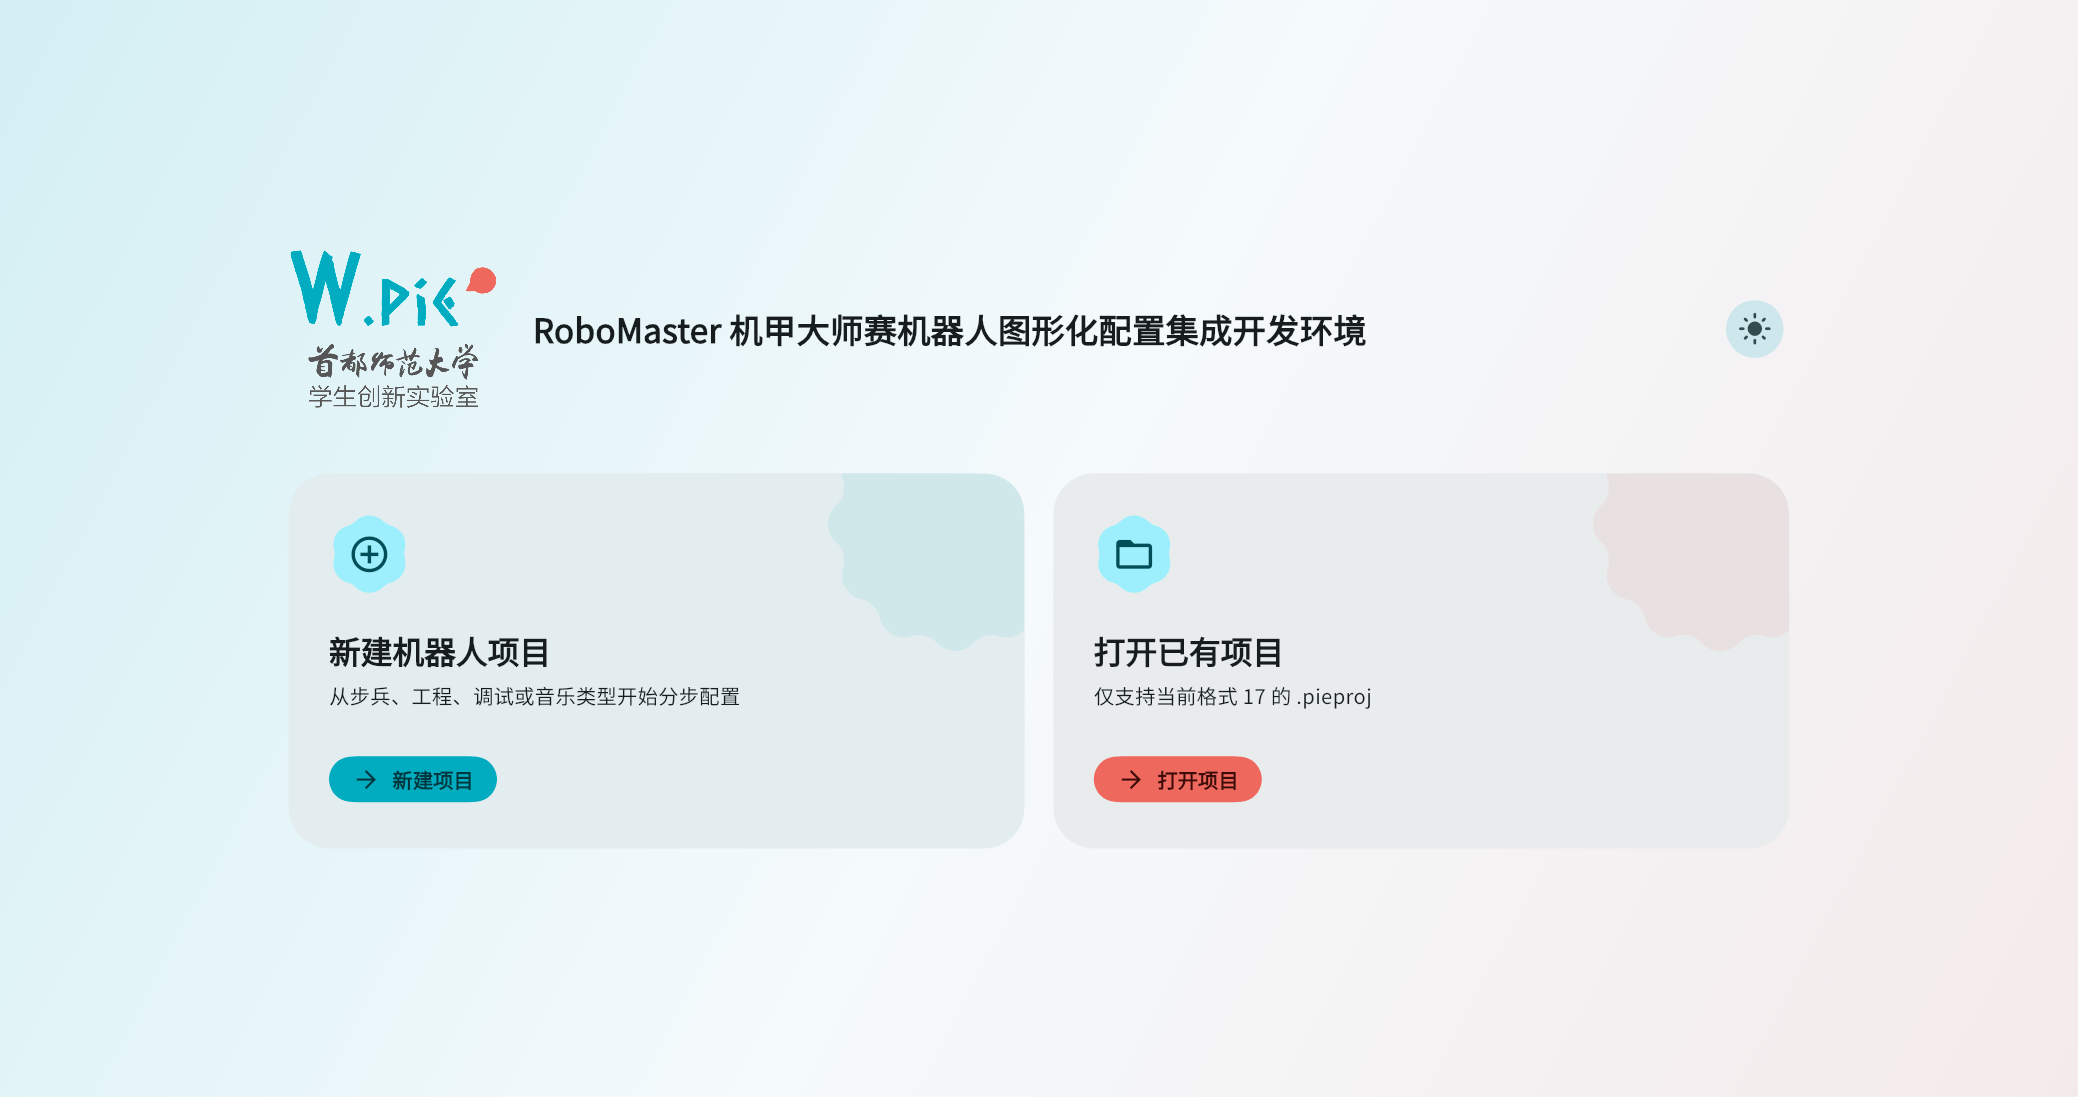
\includegraphics[width=0.9\linewidth]{image/ch01/1-1-home.png}
  \caption{PIE-Block 首页：新建机器人项目、打开已有项目与最近项目。
  所有工作围绕 \texttt{.pieproj} 项目文件展开}
  \label{fig:ch01-home}
\end{figure}

\section{项目类型与本书结构}

启动 PIE-Block，从首页“新建项目”选择四种项目类型之一（图~\ref{fig:ch01-home}）：

\begin{itemize}
  \item \textbf{步兵项目}：底盘 + 云台 + 拨弹 + 摩擦轮的标准战斗构型，
        覆盖第~\ref{ch:chassis}、\ref{ch:gimbal}~章；
  \item \textbf{工程项目}：可关掉预制底盘、用变量与受限表达式自定义
        混控与机构的开放构型，覆盖第~\ref{ch:engineer}~章；
  \item \textbf{调试项目}：十路输出逐项启停的“装车前检查单”，覆盖
        第~\ref{ch:compileflash}、\ref{ch:debugproj}~章；
  \item \textbf{音乐项目}：钢琴卷帘 + 蜂鸣器演奏，覆盖
        第~\ref{ch:music}~章。
\end{itemize}

每种项目都是一条“填参数 $\rightarrow$ 检查 $\rightarrow$ 生成代码
$\rightarrow$ 烧录”的向导流程。第~\ref{ch:gencheck}~章讲生成与检查的
机制，第~\ref{ch:linkdebug}~章深入编译、HEX 与 USB-HID 烧录，
第~\ref{ch:projects}~章讲项目文件与排障。全书示例工程都在随书仓库的
\texttt{book/examples/} 下，可直接导入对照。

\begin{table}[htbp]
  \centering
  \small
  \begin{tabular}{@{}lll@{}}
    \toprule
    随书示例 & 项目类型 & 用在 \\
    \midrule
    \texttt{infantry-standard.pieproj} & 步兵 & 第 \ref{ch:chassis}、\ref{ch:gimbal}、\ref{ch:gencheck}、\ref{ch:linkdebug} 章 \\
    \texttt{mecanum4.pieproj} & 工程 & 第 \ref{ch:engineer} 章 \\
    \texttt{omni3.pieproj} & 工程 & 第 \ref{ch:engineer} 章 \\
    \texttt{arm2dof.pieproj} & 工程 & 第 \ref{ch:engineer} 章 \\
    \texttt{debug-checklist.pieproj} & 调试 & 第 \ref{ch:compileflash}、\ref{ch:debugproj} 章 \\
    \texttt{music-twinkle.pieproj} & 音乐 & 第 \ref{ch:music} 章 \\
    \bottomrule
  \end{tabular}
  \caption{随书示例工程一览}
  \label{tab:ch01-examples}
\end{table}

